\documentclass{pgnotes}

\title{Queues (SQS)}

\begin{document}

\maketitle

\section{Message queue fundamentals}

Messaging queues are a very useful architectural component in many software systems, \autoref{fig:message-queue-components}.
They can be implemented in many different ways, but the basic ideas remain the same.

\begin{figure}[htbp]
  \centering
  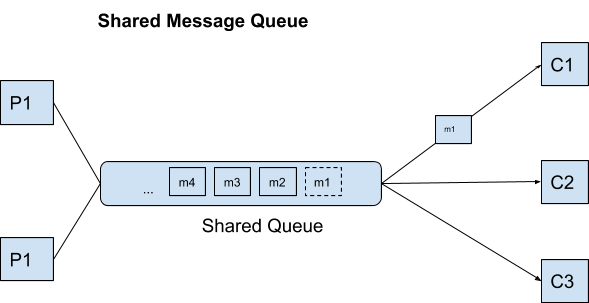
\includegraphics[width=0.75\linewidth]{shared_message_queue}
  \caption{Message queue components}
  \label{fig:message-queue-components}
\end{figure}

\subsection{Components}

\begin{description}
\item[Message:] a piece of data.  Could be text (plain, CSV, XML, JSON) or binary (JPEG, audio etc). May have also have attached meta-data. Messages are opaque from SQS.
\item[Queue:] a container for related messages and applications
\item[Producer:] connects to and places messages into the queue. Producers need not be identical to each other.
\item[Consumer:] connects to to and removes messages from the queue. Normally assume that consumers are identical to each other.
\item[Broker:] server software that creates queues and listens for connection from producers and consumers.
\end{description}
Note that there can be none, one or many producers and similarly none, one or many consumers attached to the queue at any one time. 


\subsection{Characteristics}

\begin{description}
\item[Pull model:] consumers connect to the queue and pull messages from it. (This differs from notification systems like SNS topics where messages are pushed to the subscribers.)
\item[Ordering:] how does the queue affect the order that messages are delivered in:
  \begin{description}
  \item[First-in first-out (FIFO):] where messages progress through the queue in the order they entered it in.
  \item[Priority:] where messages are ranked and highest-priority messages are delivered first.
  \item[Non-specific:] where messages are delivered generally in a FIFO manner but may not always be.
  \end{description}
\item[Durability:] said to be durable if the messages in the queue survive restarting the broker. software.
\item[Time To Live (TTL):] if a message remains in the queue longer than the specified time-to-live, then it is discarded.  (May be set at a queue level and/or at a message level.)
\item[Re-try / visibility timeouts:] what happens if a consumer takes a message and then fails when processing it. Some queues offer features to help re-deliver it.
\end{description}

\subsection{Use cases}

\begin{itemize}
\item \textbf{Triggering actions} when something else occurs.  Remember that a message in a queue needn't contain all the data about something - often it's just enough to point to data held elsewhere (such as a DBMS).
\item \textbf{Producer and consumer operate asynchronously} of each other. No need for producer to wait for consumer to process message. (Fundamental difference to a service architecture / API)
\item \textbf{Consumer may be offline} for short or long periods.  Consumer will catch-up when online again. \begin{itemize}
  \item Very useful tool for systems where a central (cloud / data-centre-based) component communicates with a remote component over a poor / intermittent connection.
  \end{itemize}
\item \textbf{Decoupling of producer and consumer}: both may be written in different languages, run on different operating systems etc. Only requirements is that they both implement the required protocol so can connect to queue via broker.
\end{itemize}

\section{SQS}

AWS provides a number of queue options: one of them is Simple Queue Service (SQS), the key features of which are shown in \autoref{fig:sqs-architecture}.

\begin{figure}[htbp]
  \centering
  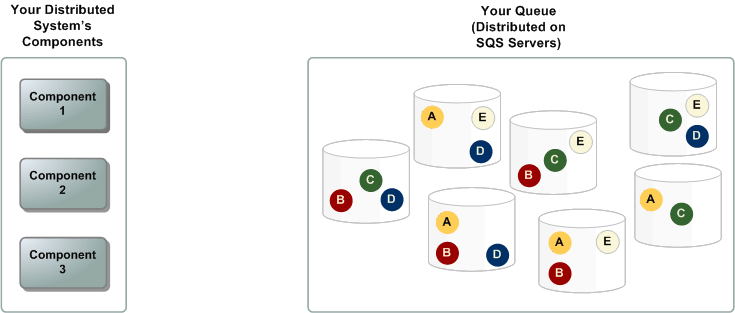
\includegraphics{sqs_architecture}
  \caption{SQS architecture}
  \label{fig:sqs-architecture}
\end{figure}

SQS queues are created thus:
\begin{minted}{powershell}
# create queue (using defaults) named labq
aws create-queue --queue-name labq

# create queue and capture queue URL in PowerShell
$QueueUrl=(aws create-queue --queue-name labq | ConvertFrom-Json).QueueUrl
# note the format of the Queue URL (it includes your account ID)
\end{minted}

\subsection{Key SQS characteristics}

\begin{itemize}
\item Protocol is HTTP-based and integrated into AWS CLI and SDK. Easily integrated into different programs.
\item Producers and consumers can be programs on your own devices / servers and/or AWS components like Lambda.
\item Queue contents are distributed across multiple servers by AWS to ensure redundancy.
\item Offered as Platform-as-a-service, so no need to consider broker and underlying components.
\item Queues can either be FIFO or ``standard queues'' where ordering may vary.
\item A given message may sometimes be received by more than one consumer. May need to plan logic.
\end{itemize}

\subsection{Sending a message}

\begin{minted}{powershell}
# show command help (to learn options)
aws sqs send-message help

# send a message to a queue given its Queue URL is in $QueueUrl
aws sqs send-message --queue-url $QueueUrl --message-body "HELLO."
# response shows message ID and MD5 hash of message body

# parse the return into PowerShell variables
$SendResult=(aws sqs send-message `
--queue-url $QueueUrl `
--message-body "HELLO." `
| ConvertFrom-Json)

# send a message from file hello.txt to a queue
aws sqs send-message --queue-url $QueueUrl --message-body file://hello.txt
\end{minted}


\subsection{Receiving a message}

\begin{minted}{powershell}
# show command help (first stop always!)
aws sqs receive-message help

# receive message from $QueueUrl
aws sqs receive-message --queue-url $QueueUrl 

# capturing as PS vars
$Messages=(aws sqs receive-message --queue-url $QueueUrl | ConvertFrom-Json).Messages
\end{minted}

Can allow multiple messages to be received in a batch (up to 10):
\begin{minted}{powershell}
# receive up to 5 messages in one operation
$Messages=(aws sqs receive-message `
--queue-url $QueueUrl `
--max-number-of-messages 5 
| ConvertFrom-Json).Messages

# number of messages received
\end{minted}

\subsection{Visibility Timeout}

Consumers receive messages off the queue and process them.
A consumer might receive a message but fail to process it correctly.
Therefore SQS has the idea of a visibility timeout, where receiving and deleting the message are two different operations.

\begin{figure}[htbp]
  \centering
  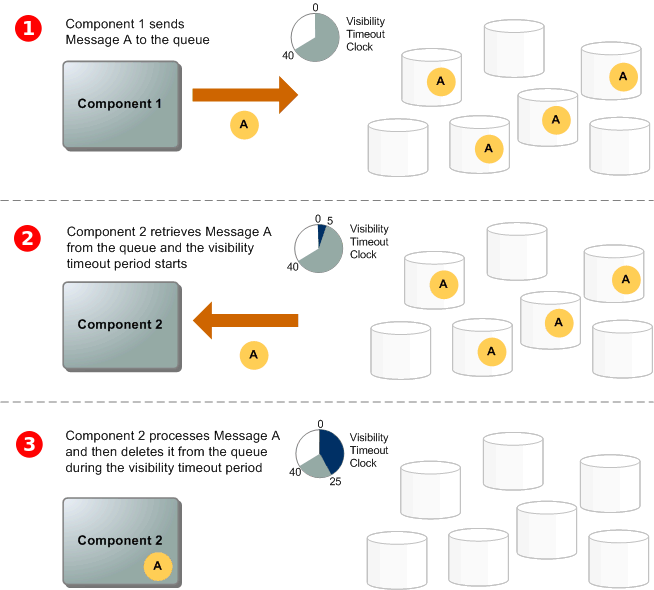
\includegraphics{sqs_message_lifecycle}
  \caption{Consumer processing message with Visiblity timeout}
  \label{fig:visibility-timeout-processing}
\end{figure}

Sequence: 
\begin{enumerate}
\item Consumer receives next message from queue. This makes the message invisible to other consumers for the set visibility timeout. Any receive calls will receive other/no messages.
\item Consumer attempts to process the message.
\item If the message is processed successfully, consumer deletes it from queue. (Last step for consumer)
\item If the consumer fails to process the message, crashes etc. it will not get as far as deleting the message from the queue. The message will then re-appear for consumption.
\end{enumerate}

\begin{minted}{powershell}
# receive message
$Message=$(aws sqs receive-message `
--queue-url $QueueUrl 
| ConvertFrom-Json).Messages 

# process the message

# then delete using its receipt handle
aws sqs delete-message --queue-url $QueueUrl --receipt-handle $Message.ReceiptHandle
\end{minted}

Of course, can avoid this behaviour by just deleting message immediately on receipt.

The default visibility timeout is 30 seconds.
Can be set for queue by modifying queue attributes:
\begin{minted}{powershell}
aws sqs set-queue-attributes `
--queue-url $QueueUrl `
--attributes VisibilityTimeout=3600
\end{minted}

\subsection{Retention period}

Messages remaining in the queue longer than the Retention Period are automatically deleted.
\begin{minted}{powershell}
# set retention period to 1 hour (=60*60 seconds)
aws sqs set-queue-attributes `
--queueurl $QueueUrl `
--attributes MessageRetentionPeriod=3600
\end{minted}

\subsection{Introduce a delay}

Messages can be delayed from being received after being sent to queue:
\begin{minted}{powershell}
# keep messages back for 60 seconds
aws sqs set-queue-attributes `
--queueurl $QueueUrl `
--attributes DelaySeconds=60
\end{minted}

\subsection{Purging a queue}

Purging a queue removes all messages from it.
\begin{minted}{powershell}
aws sqs purge-queue --queue-url $QueueUrl
\end{minted}


\section{Exercise}

\begin{enumerate}

\item Create a queue called labq.
  
\item Use PowerShell to construct a producer and consumer.
  The consumer should take some action on the message (e.g. print to screen, write to file).
  Build a time-delay into the consumer to simulate processing.

\item Create an S3 bucket.
  Modify your consumer to put each message as a new object into the S3 bucket.
  Write a script that loops over the S3 bucket and prints the messages.
  
\item
  Optional: replace / augment the PowerShell producer or consumer with an equivalent in another language.

\end{enumerate}


\end{document}
